\chapter{Auswertung}\label{cha:auswertung}
\section{Ausgehobene Daten}\label{sec:aushebungDaten}
Dieses Kapitel soll zeigen wie genau das Ergebnis für eine Elementarladung wurde. Für das muss aber zuerst ein Blick auf die Daten gemacht werden, die herausgekommen sind beim Experimentieren. In der \autoref{tab:ergebnisse} befinden sich die Spalten, Steig und Fallgeschwindigkeit, Radius, Masse und Ladung des Tröpfchens. Eine vollständige Messtabelle befindet sich im Anhang. Dort werden auch Messungen aufgeführt, die nicht gut genug waren. Sie wurden bei den Berechnungen nicht berücksichtigt. Diese Daten können jetzt auf ein Punktdiagramm gezeichnet werden. Dabei soll die Y-Achse die Ladung der Tröpfchen sein und die X-Achse die jeweilige Nummerierung. Das Diagramm wurde mit Microsoft Excel erstellt und sieht folgendermassen aus.

\begin{figure}[h]
	\centering
	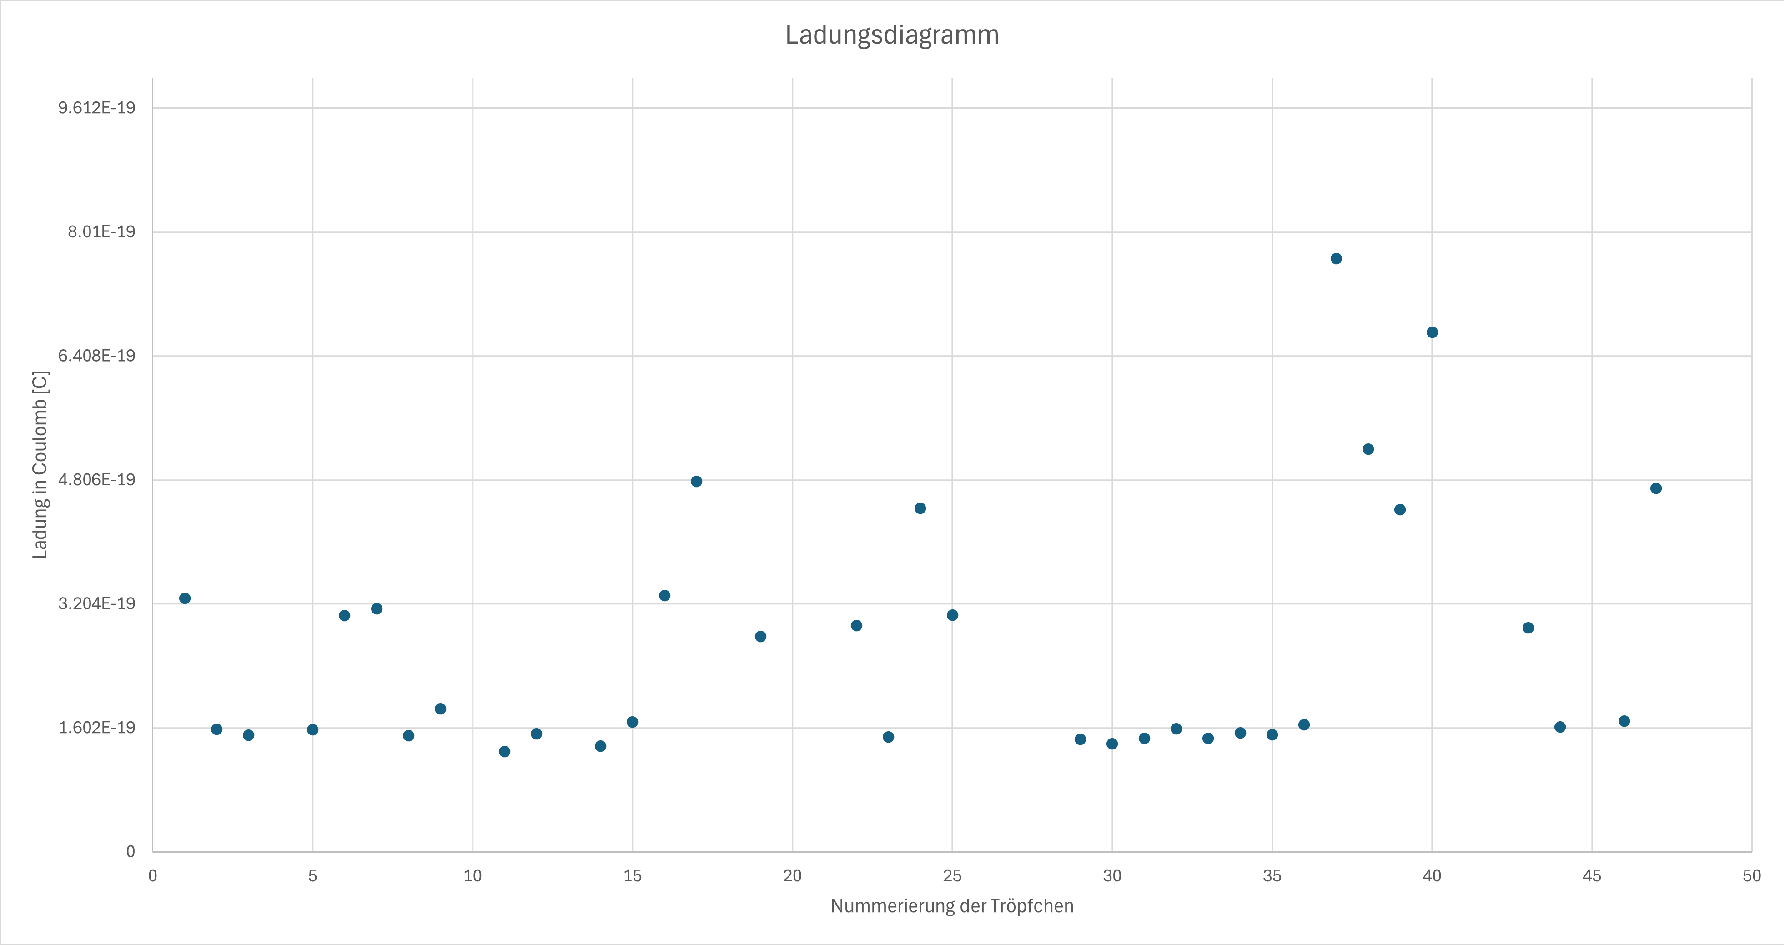
\includegraphics[width=\textwidth]{bilder/pdf/LadungsdiagrammOhne.pdf}
	\caption{Ladungsdiagramm ohne Fehlerrechnung}
	\label{fig:ladungsdiagrammOFehlerrechnung}
\end{figure}

Die Abstände auf der Y-Achse sind nicht zufällig gewählt, sondern ein Linienabstand entspricht exakt einer Elementarladung. Jetzt kann abgelesen werden, wie viele Elementarladungen jedes einzelne Tröpfchen hatte. Es war überraschend zu sehen, wie genau das Experiment geklappt hat. Man sieht, wie sich die Ladungen in Stufen anordnen. Während dem Experimentieren hätte man das nie gedacht. In \autoref{sec:genauigkeitAuswertung} geht man noch auf die Genauigkeit aller Ergebnisse ein, mithilfe einer Fehlerrechnung. Während dem Experimentieren und Auswerten gab es keinen einzigen Sonderfall, der eine viel zu hohe oder tiefe Ladung ergab, das überraschte auch, denn das Experiment hängt von sehr vielen verschiedenen Faktoren und Messgrössen ab.

\section{Das Ergebnis}\label{sec:ergebnis}
In der \autoref{tab:ergebnisse} kann jetzt eine weitere Spalte hinzugefügt werden, die Anzahl der Elementarladungen $n$. Wenn das hinzugefügt wurde sehen die ersten 10 Zeilen so aus:

\begin{table}[H]
	\centering
	\begin{tabular}{llllll|l}
		\toprule
		Nr. & $v_{rise}$ & $v_{fall}$ & Radius & Masse & Ladung & Anzahl (n) \\
		\midrule
		1 &$\mathrm{2.01 \cdot 10^{-04}}$ & $\mathrm{2.12 \cdot 10^{-05}}$ & $\mathrm{4.04 \cdot 10^{-07}}$ & $\mathrm{2.45 \cdot 10^{-16}}$ & $\mathrm{3.27 \cdot 10^{-19}}$ & 2\\
		2 &$\mathrm{8.46 \cdot 10^{-05}}$ & $\mathrm{2.16 \cdot 10^{-05}}$ & $\mathrm{4.08 \cdot 10^{-07}}$ & $\mathrm{2.53 \cdot 10^{-16}}$ & $\mathrm{1.59 \cdot 10^{-19}}$ & 1\\
		3 &$\mathrm{8.68 \cdot 10^{-05}}$ & $\mathrm{1.98 \cdot 10^{-05}}$ & $\mathrm{3.90 \cdot 10^{-07}}$ & $\mathrm{2.20 \cdot 10^{-16}}$ & $\mathrm{1.51 \cdot 10^{-19}}$ & 1\\
		4 &$\mathrm{8.91 \cdot 10^{-05}}$ & $\mathrm{2.04 \cdot 10^{-05}}$ & $\mathrm{3.96 \cdot 10^{-07}}$ & $\mathrm{2.31 \cdot 10^{-16}}$ & $\mathrm{1.58 \cdot 10^{-19}}$ & 1\\
		5 &$\mathrm{1.97 \cdot 10^{-04}}$ & $\mathrm{1.98 \cdot 10^{-05}}$ & $\mathrm{3.89 \cdot 10^{-07}}$ & $\mathrm{2.18 \cdot 10^{-16}}$ & $\mathrm{3.05 \cdot 10^{-19}}$ & 2\\
		6 &$\mathrm{1.98 \cdot 10^{-04}}$ & $\mathrm{2.04 \cdot 10^{-05}}$ & $\mathrm{3.96 \cdot 10^{-07}}$ & $\mathrm{2.31 \cdot 10^{-16}}$ & $\mathrm{3.14 \cdot 10^{-19}}$ & 2\\
		7 &$\mathrm{9.33 \cdot 10^{-05}}$ & $\mathrm{1.84 \cdot 10^{-05}}$ & $\mathrm{3.74 \cdot 10^{-07}}$ & $\mathrm{1.95 \cdot 10^{-16}}$ & $\mathrm{1.50 \cdot 10^{-19}}$ & 1\\
		8 &$\mathrm{1.26 \cdot 10^{-04}}$ & $\mathrm{1.71 \cdot 10^{-05}}$ & $\mathrm{3.61 \cdot 10^{-07}}$ & $\mathrm{1.74 \cdot 10^{-16}}$ & $\mathrm{1.85 \cdot 10^{-19}}$ & 1\\
		9 &$\mathrm{1.12 \cdot 10^{-04}}$ & $\mathrm{1.23 \cdot 10^{-05}}$ & $\mathrm{3.01 \cdot 10^{-07}}$ & $\mathrm{1.01 \cdot 10^{-16}}$ & $\mathrm{1.29 \cdot 10^{-19}}$ & 1\\
		10 &$\mathrm{1.30 \cdot 10^{-04}}$ & $\mathrm{1.29 \cdot 10^{-05}}$ & $\mathrm{3.08 \cdot 10^{-07}}$ & $\mathrm{1.09 \cdot 10^{-16}}$ & $\mathrm{1.53 \cdot 10^{-19}}$ & 1\\
		\bottomrule
		&&&&& $2.031 \cdot 10^{-18}$ & 13 \\
	\end{tabular}
	\caption{Ergebnisse mit Anzahl Ladungen}
	\label{tab:anzahlLadung}
\end{table}
\par
\noindent Die Anzahl Elementarladungen werden zusammengerechnet und die Summe daraus beträgt 13 Elementarladungen. Dann werden die Ladungen summiert, das ergiebt $2.031 \cdot 10^{-18}$. Das arithmetische Mittel aus diesen beiden Messwerten lautet dann: $\frac{2.031 \cdot 10^{-18}}{13} \ = \ 1.56 \cdot 10^{-19} Coulomb$. 

Wenn dieser Vorgang mit allen Werten in der Tabelle gemacht wird, kommt man auf eine Anzahl von 60 Elementarladungen und einer Summe von $9.313 \cdot 10^{-18}$ Coulomb. Danach wird wieder das Mittel genommen und das Ergebnis dieser Arbeit für eine Elementarladung Lautet:

\begin{equation}\label{eq:ergebnis}
	\frac{9.313 \cdot 10^{-18}C}{60} \ = \ 1.5522 \cdot 10^{-19} Coulomb
\end{equation}

\section{Die Genauigkeit}\label{sec:genauigkeitAuswertung}
Wie genau ist ein solches Ergebnis eines Experimentes? Hier ist nun der zweite Teil der Arbeit, das Fehlerrechnen. Hier wird für jede einzelne Grösse einen absoluten und relativen Fehler bestimmt, der danach mithilfe der verschiedenen Formeln zusammengerechnet werden kann. Ein solches Experiment enthaltet Fehler, die von den Messinstrumenten oder Experimentierapparaten hervorkommen, zum Beispiel ist das Multimeter nicht richtig kalibriert oder die Gitternetzlinien sind nicht exakt 0.5 mm voneinander entfernt. Diese Fehler nennt man systematische Fehler, sie können vermieden werden, indem das Experiment sorgfältig vorbereitet wird. Die anderen Fehler, wie zum Beispiel die Reaktionszeit beim Zeitmessen, der Blickwinkel beim Beobachten oder Temperatur und Luftdruckschwankungen während dem Experimentieren, werden zufällige Fehler genannt. Sie sind schwieriger zu eliminieren, können aber durch mehrere Messungen und dadurch gezogene Durchschnittswerte, minimiert werden. 

\subsection{Fehlerrechnung}\label{sub:fehler}
Zuerst müssen für alle Messgrössen absolute Fehler entschieden werden. Die können abgeschätzt werden oder hängen von der Genauigkeit eines Messgerätes ab.

\begin{center}
	\begin{tabular}[h]{l|lll}
		& Messwert & absoluter Fehler & relativer Fehler [\%] \\
		\toprule
		Elektrisches Feld [V/m] &
	\end{tabular}
\end{center}
\begin{table}
\caption{Ergebnisse der Berechnung}
\label{tab:ergebnisse}
\begin{tabular}{lllll}
\toprule
v_rise & v_fall & Radius & Masse & Ladung \\
\midrule
2.01 \times 10^{-04} & 2.12 \times 10^{-05} & 4.04 \times 10^{-07} & 2.45 \times 10^{-16} & 3.27 \times 10^{-19} \\
8.46 \times 10^{-05} & 2.16 \times 10^{-05} & 4.08 \times 10^{-07} & 2.53 \times 10^{-16} & 1.59 \times 10^{-19} \\
8.68 \times 10^{-05} & 1.98 \times 10^{-05} & 3.90 \times 10^{-07} & 2.20 \times 10^{-16} & 1.51 \times 10^{-19} \\
8.91 \times 10^{-05} & 2.04 \times 10^{-05} & 3.96 \times 10^{-07} & 2.31 \times 10^{-16} & 1.58 \times 10^{-19} \\
1.97 \times 10^{-04} & 1.98 \times 10^{-05} & 3.89 \times 10^{-07} & 2.18 \times 10^{-16} & 3.05 \times 10^{-19} \\
1.98 \times 10^{-04} & 2.04 \times 10^{-05} & 3.96 \times 10^{-07} & 2.31 \times 10^{-16} & 3.14 \times 10^{-19} \\
9.33 \times 10^{-05} & 1.84 \times 10^{-05} & 3.74 \times 10^{-07} & 1.95 \times 10^{-16} & 1.50 \times 10^{-19} \\
1.26 \times 10^{-04} & 1.71 \times 10^{-05} & 3.61 \times 10^{-07} & 1.74 \times 10^{-16} & 1.85 \times 10^{-19} \\
1.12 \times 10^{-04} & 1.23 \times 10^{-05} & 3.01 \times 10^{-07} & 1.01 \times 10^{-16} & 1.29 \times 10^{-19} \\
1.30 \times 10^{-04} & 1.29 \times 10^{-05} & 3.08 \times 10^{-07} & 1.09 \times 10^{-16} & 1.53 \times 10^{-19} \\
1.26 \times 10^{-04} & 1.15 \times 10^{-05} & 2.89 \times 10^{-07} & 8.97 \times 10^{-17} & 1.37 \times 10^{-19} \\
1.21 \times 10^{-04} & 1.58 \times 10^{-05} & 3.45 \times 10^{-07} & 1.52 \times 10^{-16} & 1.68 \times 10^{-19} \\
2.26 \times 10^{-04} & 1.81 \times 10^{-05} & 3.72 \times 10^{-07} & 1.91 \times 10^{-16} & 3.31 \times 10^{-19} \\
4.50 \times 10^{-04} & 1.21 \times 10^{-05} & 2.97 \times 10^{-07} & 9.76 \times 10^{-17} & 4.79 \times 10^{-19} \\
2.84 \times 10^{-04} & 1.07 \times 10^{-05} & 2.76 \times 10^{-07} & 7.83 \times 10^{-17} & 2.79 \times 10^{-19} \\
2.43 \times 10^{-04} & 1.40 \times 10^{-05} & 3.23 \times 10^{-07} & 1.25 \times 10^{-16} & 2.93 \times 10^{-19} \\
1.26 \times 10^{-04} & 1.28 \times 10^{-05} & 3.07 \times 10^{-07} & 1.07 \times 10^{-16} & 1.48 \times 10^{-19} \\
3.97 \times 10^{-04} & 1.30 \times 10^{-05} & 3.10 \times 10^{-07} & 1.11 \times 10^{-16} & 4.44 \times 10^{-19} \\
2.49 \times 10^{-04} & 1.45 \times 10^{-05} & 3.29 \times 10^{-07} & 1.32 \times 10^{-16} & 3.06 \times 10^{-19} \\
3.96 \times 10^{-05} & 3.36 \times 10^{-05} & 5.20 \times 10^{-07} & 5.22 \times 10^{-16} & 1.46 \times 10^{-19} \\
1.04 \times 10^{-04} & 1.47 \times 10^{-05} & 3.31 \times 10^{-07} & 1.35 \times 10^{-16} & 1.40 \times 10^{-19} \\
5.22 \times 10^{-05} & 2.89 \times 10^{-05} & 4.79 \times 10^{-07} & 4.08 \times 10^{-16} & 1.47 \times 10^{-19} \\
5.40 \times 10^{-05} & 3.06 \times 10^{-05} & 4.95 \times 10^{-07} & 4.50 \times 10^{-16} & 1.59 \times 10^{-19} \\
5.82 \times 10^{-05} & 2.67 \times 10^{-05} & 4.59 \times 10^{-07} & 3.60 \times 10^{-16} & 1.46 \times 10^{-19} \\
5.34 \times 10^{-05} & 2.98 \times 10^{-05} & 4.88 \times 10^{-07} & 4.30 \times 10^{-16} & 1.54 \times 10^{-19} \\
5.76 \times 10^{-05} & 2.79 \times 10^{-05} & 4.71 \times 10^{-07} & 3.87 \times 10^{-16} & 1.52 \times 10^{-19} \\
5.81 \times 10^{-05} & 3.01 \times 10^{-05} & 4.91 \times 10^{-07} & 4.38 \times 10^{-16} & 1.64 \times 10^{-19} \\
5.32 \times 10^{-04} & 1.89 \times 10^{-05} & 3.81 \times 10^{-07} & 2.06 \times 10^{-16} & 7.67 \times 10^{-19} \\
3.55 \times 10^{-04} & 1.90 \times 10^{-05} & 3.82 \times 10^{-07} & 2.06 \times 10^{-16} & 5.21 \times 10^{-19} \\
3.31 \times 10^{-04} & 1.65 \times 10^{-05} & 3.54 \times 10^{-07} & 1.64 \times 10^{-16} & 4.42 \times 10^{-19} \\
4.85 \times 10^{-04} & 1.78 \times 10^{-05} & 3.68 \times 10^{-07} & 1.85 \times 10^{-16} & 6.71 \times 10^{-19} \\
2.10 \times 10^{-04} & 1.66 \times 10^{-05} & 3.55 \times 10^{-07} & 1.66 \times 10^{-16} & 2.89 \times 10^{-19} \\
1.04 \times 10^{-04} & 1.77 \times 10^{-05} & 3.67 \times 10^{-07} & 1.83 \times 10^{-16} & 1.61 \times 10^{-19} \\
2.14 \times 10^{-04} & 7.96 \times 10^{-06} & 2.34 \times 10^{-07} & 4.75 \times 10^{-17} & 1.69 \times 10^{-19} \\
6.02 \times 10^{-04} & 8.06 \times 10^{-06} & 2.36 \times 10^{-07} & 4.85 \times 10^{-17} & 4.70 \times 10^{-19} \\
\bottomrule
\end{tabular}
\end{table}
